% asset_id: FAS1ComplexNumbersLociRegionsTikZ-002
\documentclass[tikz,border=8pt]{standalone}
\usepackage{amsmath}
\usepackage{xcolor}
\definecolor{Canvas}{HTML}{FAF9F6}
\definecolor{Ivory}{HTML}{FFFFF0}
\definecolor{SoftLine}{HTML}{E5E5EA}
\definecolor{TextInk}{HTML}{2C2C2E}
\definecolor{Gold}{HTML}{C5A059}
\definecolor{BrightGold}{HTML}{D4AF37}
\begin{document}
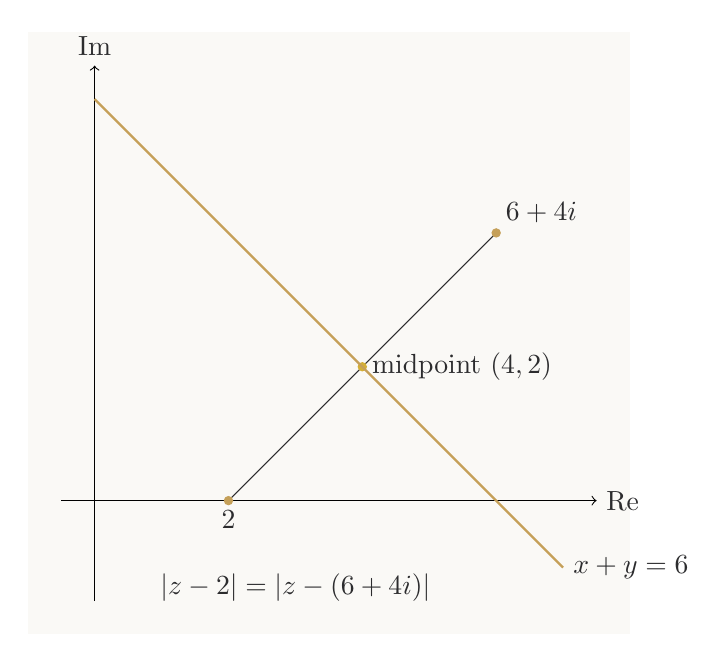
\begin{tikzpicture}[scale=0.85,every node/.style={text=TextInk}]
\fill[Canvas] (-1,-2) rectangle (8,7);
\draw[->] (-.5,0)--(7.5,0) node[right] {$\operatorname{Re}$};
\draw[->] (0,-1.5)--(0,6.5) node[above] {$\operatorname{Im}$};
\coordinate (A) at (2,0);\coordinate (B) at (6,4);\coordinate (M) at (4,2);
\draw[TextInk] (A)--(B);
\fill[Gold] (A) circle (2pt) node[below] {$2$};
\fill[Gold] (B) circle (2pt) node[above right] {$6+4i$};
\fill[BrightGold] (M) circle (2pt) node[right] {midpoint $(4,2)$};
\draw[Gold,thick] (0,6)--(7,-1) node[right] {$x+y=6$};
\node at (3,-1.3) {$\lvert z-2\rvert=\lvert z-(6+4i)\rvert$};
\end{tikzpicture}
\end{document}
